\title{Arch Linuxのインストール}
\author{おがわ}
\begin{document}
  \begin{frame}
    \note {
      動画全体ので説明する項目概要\\
      用語について、随時説明を加えています。
    }
    \frametitle{Arch Linuxのインストール}
    \begin{enumerate}
      \item ハードウェア、ファーム(UEFI)の仕様
        \note [item] {
          OSのインストーラソフト(Arch linux)は、ファーム(UEFI)の仕様に従いハードウェアを認識します。仕様を理解しておくと、動作しない場合の対策を立てやすくなります。
        }
      \item OSのファイルシステム
        \note [item] {
          ストレージデバイス(ssd)のパーティション設定、各パーティションのファイルフォーマットの選定と設定をおこないます。
        }
      \item Linuxのインストールからネットワークの接続設定(wifi)
        \note [item] {
          インストーラソフトによるストレージデバイスへのLinuxカーネルと必要なソフトウェアのインストールを行います。
          ネットワーク接続設定のためのソフトウェアの選定、インストールを行います。
        }
    \end{enumerate} 
  \end{frame}
  \begin{frame}
    \frametitle{ハードウェア構成}
    \note{
      インストール対象のハードウェアは次のとおりです。
    }
    \begin{center}
      \begin{tabular}{l|l}
        \hline
        cpu & AMD Ryzen7 8845HS \\ \hline
        memory & 64 GB \\  \hline
        ssd & 2 TB \\ \hline
        グラフィック& Radeon 780M \\
        \hline
      \end{tabular} \\
    \end{center}
    \note[item]{cpuはAMD Ryzen7。本体の裏面の蓋を開けた状態の画像からは確認できません。} 
    \note[item]{memoy 32GBのメモリカード2枚で64GB}
    \note[item]{ストレージはssdで、2TBを設置}
    \note[item]{グラフィックはRadeon。こちらも画像からは確認できません。}
  \end{frame}
  \begin{frame}
    \frametitle{入出力ポート} 
    \note{
      入出力ポートについては、次のものが利用できます。
    }
    \begin{center}
      \begin{tabular}{l|l|l}
        \hline
        USB 3.2 & 2 & \\ \hline
        USB 2.0 & 2 & \\ \hline
        HDMI & 2 & \\ \hline
        シリアルポート & 1 & RS232、RS485 \\
        \hline
      \end{tabular}
      \note[item] {USB3.2のタイプAのポートが2つ。位置は前面}
      \note[item] {USB2.0のタイプAのポートが2つ。位置は背面}
      \note[item] {HDMIのポートが2つ。位置は背面}
      \note[item] {シリアルのポートが1つ。位置は背面。今すぐの利用は考えていません。}
    \end{center}
  \end{frame}
  \begin{frame}
    \frametitle{ネットワーク} 
    \note{
      ネットワーク関連は、表のようになっています。
    }
    \begin{center}    
      \begin{tabular}{l|l}
        \hline
        イーサネット& 2 \\ \hline
        Wi-Fi & 1 \\
        \hline
      \end{tabular}
      \note[item] {イーサネットポートが2つ。位置は背面}
      \note[item] {Wi-Fiが1つ。アンテナが背面に確認できます}
    \end{center}
  \end{frame}
  \begin{frame}
    \frametitle{ファーム}
    \note{AMI社のファームで、UEFI仕様に従っています。}
    \begin{center}
    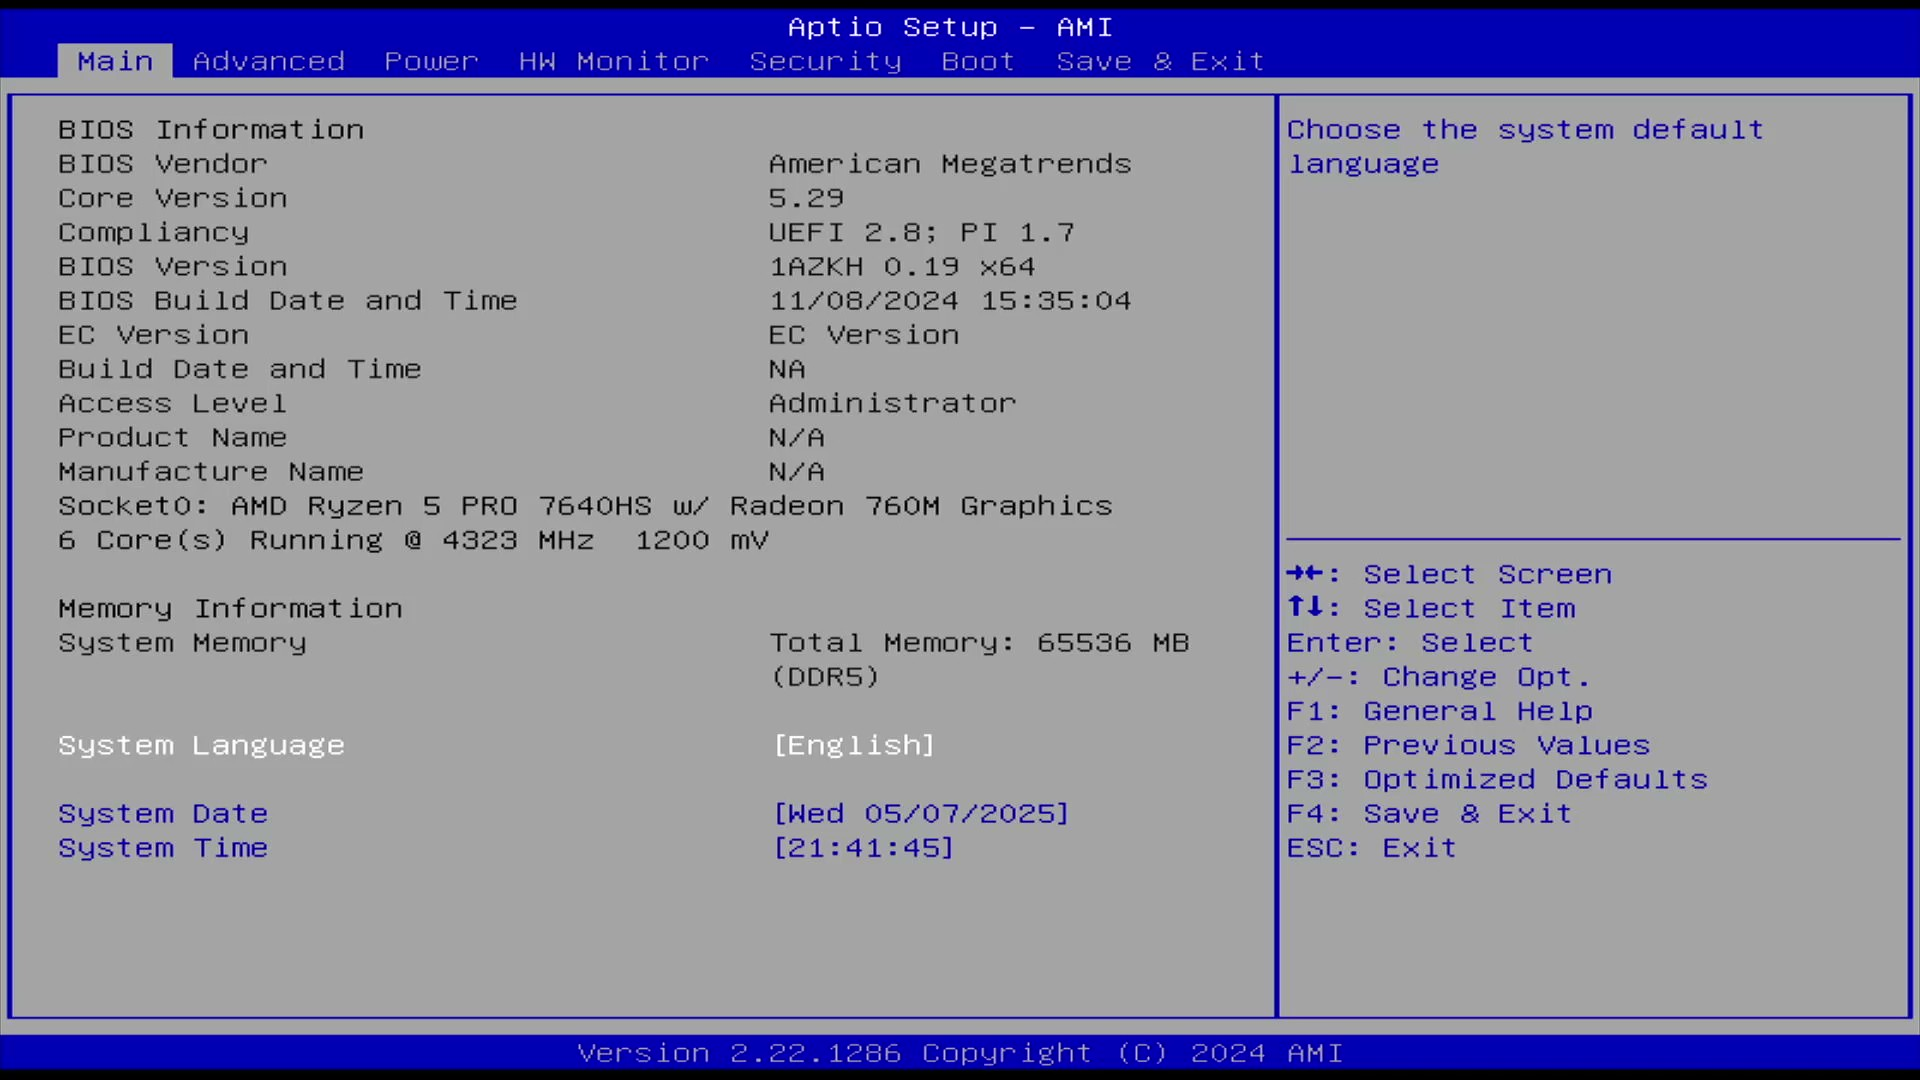
\includegraphics[height=5cm]{img/bios-display-1.jpg}
    \end{center}
  \end{frame}
\end{document}
% vi: se ts=2 sw=2 et:
